\chapter{Implementation}
\label{chapter:implementation}
Make some general points here

\section{Getting Started}

\subsection{Require.js}
When the GatePlay url is visited, the only file downloaded is the main HTML file: index.html. The index then directs the user's browser to download the additional CSS and JavaScript files needed to use GatePlay.

A JavaScript script may use methods or variables defined in the global namespace, even if they were put there by another script, provided that the script has already been run.

\begin{figure}[H]
\begin{lstlisting}[language=html]
<!-- componentview depends on component -->
<!-- Therefore we ensure component is loaded first -->
<script type="text/javascript" src=".../component.js"></script>
<script type="text/javascript" src=".../componentview.js"></script>
\end{lstlisting}
\caption{Example use of Script tags}
\end{figure}

It is time consuming for a human to find and type out a correct ordering for the Script tags, and it would need to be updated every time a file as added or removed, or sometimes if a file were modified.

Require.js is a JavaScript file loader which does automatically loads files in a correct order. Each JavaScript file declares each of its direct dependencies, and Require.js will ensure they are all loaded correctly when the webpage loads.

\begin{figure}[H]
\begin{lstlisting}[language=JavaScript]
// componentview.js

require([
	// Declare the path of each file we require	
	"canvas/model/component"
], function(Component) {
	// Each included file is run, and we can give a name to whatever it returns if desired
	var myComponent = new Component();
	...
});
\end{lstlisting}
\caption{An example file which uses Require.js}
\end{figure}

\section{The Workbench}

GatePlay's workbench is where we create and view circuits, and is implemented using an HTML Canvas element. A canvas is a blank slate which can have shapes and images drawn using the JavaScript API.


\subsection{Fabric.js}
An HTML Canvas only provides low level drawing tools. You are able to draw shapes and images on it, but there is no concept of persist objects on the canvas.

Fabric.js is a library which wraps HTML Canvases with an object model, allowing GatePlay to interact at the level of objects being added to, modified, and remove from the canvas, rather thana  flat array of pixels.

Suppose I wanted to add a rectangle to a canvas, and then move it to a new location. Using Fabric.js this is two library calls (one to add a rectangle object and one to change the position property of the object). Using an HTML Canvas it is still one call to draw the rectangle, but moving it would require calculating what would be behind the rectangle, drawing that over the rectangle, and then re-drawing the rectangle at its new location. Fabric.js greatly reduces the amount of boilerplate code otherwise needed to interact with canvases.

Initially GatePlay used a different canvas framework called KineticJS, but due to difficulties getting features like snap-to-grid working I switched to Fabric.js.

\subsection{MVC with Backbone.js}
Model-view-controller\footnote{http://en.wikipedia.org/wiki/Model-view-controller} is a design pattern to simply program development. GatePlay uses MVC in the implementation of the workbench. MVC applications contain three types of components:

\begin{itemize}
	\item \textbf{Models} which store some part of the state of the application
	\item \textbf{Views} which display a representation of one of the models to the user
	\item \textbf{Controllers} which process user input, and updates the appropriate models.
\end{itemize}

The interactions between the components can be seen in figure~\ref{fig:mvc}. By separating out the concerns of the program it becomes possible to, for example, add new views for your models without needing to change the models or controllers themselves.

\begin{figure}[H]
	\centering
	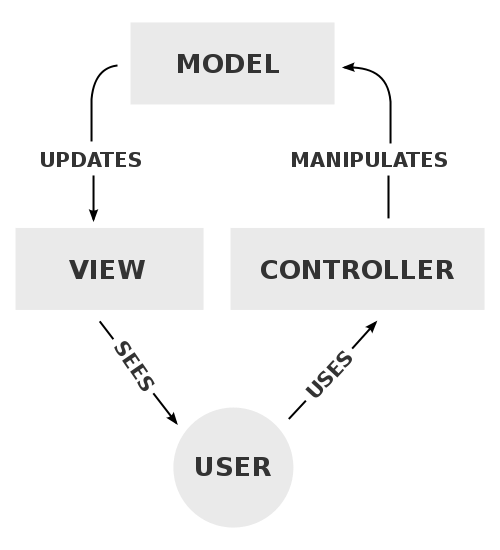
\includegraphics[width=0.5\textwidth]{mvc.png}
	\caption{Interaction of MVC Components, from Wikipedia}
	\label{fig:mvc}
\end{figure}

Backbone.js\footnote{http://backbonejs.org} is a JavaScript library to reduce the amount of boilerplate code in developing MVC JavaScript applications.

One model is the Wire model as shown in figure~\ref{fig:wiremodel}. It includes a lot of the same information as the Wire objects used in the simulation, but also includes information regarding the \textit{fixed points} of the wire.

We then create a view associated with the Wire model (figure~\ref{fig:wireview}). 

\begin{figure}
\begin{lstlisting}[language=JavaScript]
Backbone.Model.extend({
	defaults: function() {
    	return {
        	id: nextWireId++,
        	sourceId: -1,
        	sourcePort: -1,
       	 	targetId: -1,
        	targetPort: -1,
        	fixedPoints: [],
        	truthValue: TruthValue.UNKNOWN
    	}
	},
})
\end{lstlisting}
caption{Definition of a Wire model}
\label{fig:wiremodel}
\end{figure}

\begin{figure}
\begin{lstlisting}[language=JavaScript]
Backbone.View.extend({
    initialize: function(options) {
        // When the model is changed, update the view
        this.model.on("change:fixedPoints", this.render, this);
        this.model.on("change:truthValue", this._setWireColor, this);
    },

    render : function() {
        var model = this.model;
		
		// Using the model data we can now draw wires on the canvas
    },

    _setWireColor: function() {
        var truthValue = this.model.get("truthValue");
        
        // We can now re-render the wire with the new colour
    }
});
\end{lstlisting}
caption{Definition of a Wire view}
\label{fig:wireview}
\end{figure}


\subsection{Editing Mode}


\subsection{Running Mode}

\section{The Simulator}
The implementation of GatePlay's simulator is a relatively straightforward implementation of the algorithms and ideas explained in section~\ref{chapter:simulation}. The following six classes fully implement the simulator:

\begin{itemize}
	\item \textbf{truthvalue.js} defines constants $True$, $False$, and $Unknown$
	\item \textbf{component.js} defines a Component by its input count, output count, and evaluation function
	\item \textbf{wire.js} defines a Wire by its input component and port, output component and port, and truth value
	\item \textbf{circuitevent.js} defines a CircuitEvent by component, port, timestamp, and value
	\item \textbf{functions.js} contains definitions of all the Evaluation Functions available to the simulator 
	\item \textbf{circuit.js} is the only class which need be visible from outside the simulator. It has an interface to add components and wires. Circuit.js implements the algorithm for the event loop. 
\end{itemize}

\subsection{Blinker Events}
Recall section~\ref{subsec:initial} that $Blinker$ components toggle their output value at a set interval. Each $Blinker$ has its own, potentially unique, interval.

To implement this, a $Blinker$ component's evaluation function (shown in figure~\ref{fig:blinkereval} determines it truth value backed on the simulation clock.

\begin{figure}
\begin{lstlisting}[language=JavaScript]
Blinker.prototype._doEvaluate = function(argList, clock) {
    var period = Math.floor(clock / this._interval);
    var parity = period % 2;
    if (parity === 0) {
        return [TruthValue.TRUE];
    } else {
        return [TruthValue.FALSE];
    }
};
\end{lstlisting}
\caption{Implementation of $Blinker$'s evaluation function}
\label{fig:blinkereval}
\end{figure}

However a $Blinker$ will never be processed by the event loop, as no events will ever affect a $Blinker$ (it has no inputs). Therefore we need to handle $Blinker$s differently.

The solution implemented in GatePlay is to add a new circuit event for every $Blinker$, \textit{every} clock tick. For a $Blinker$ with interval $2$, we would add $True$ events at time $0$ and $1$, $False$ events at time $2$ and $3$, and so on. We rely on culling to eliminate the replicated events.

The algorithm described above if very easy to implement, but clearly inefficient if there were a large number of $Blinker$s. A better algorithm where we only add one circuit event per $Blinker$, per interval is outlined in figure~\ref{fig:blinkerqueue}. 

\begin{figure}
\begin{lstlisting}[language=JavaScript]
function tick() {
	// For each event which is happening at this time
	while (this._blinkerEventQueue.peek().time <= this._clock) {
		var event = this._blinkerEventQueue.pop();
		this._addEvent(event);
		
		var blinker = this.getComponent(event.sourceId);
		var nextTime = event.eventTime + blinker.get("interval");
		var nextValue = blinker.evaluate([], nextTime);
		var nextEvent = new CircuitEvent(nextTime, event.sourceId, event.sourcePort, nextValue);
	}
	
	// Event loop goes here
}
\end{lstlisting}
\caption{}
\label{fig:blinkerqueue}
\end{figure}

Note that the \textit{blinkerEventQueue} is just a subset of the main event queue, and we could actually put this algorithm directly in the event loop. However doing so would couple our implementation of the general event queue with that of a specific type of component and not be good software engineering practice.

\section{Drag-and-drop}
One of the requirements of GatePlay was that it be easy to use, and the drag-and-drop nature of the interface is an important part of that. Implementing drag-and-drop is can be split in to three main sub problems:

\begin{enumerate}
	\item Drawing the components in the left-bar
	\item Allow dragging components from the left side-bar
	\item Adding components to the workbench where they dropped
\end{enumerate}

We first create an HTML Image element for each component on the left-bar. The matter of creating images for each component is handled by the  \textit{createThumbnail} function. \textit{createThumbnail} creates a temporary canvas for each component and renders the component on it. This canvas can be converted to an image file by Fabric.js.

jQueryUI\footnote{http://http://jqueryui.com/} is a JavaScript library to ease the creation of interactive web applications like GatePlay. jQueryUI supports \textit{Draggable} and \textit{Droppable} interactions, which implement exactly what we want. The components in the left-bar are marked as Draggable and the main workbench is marked as Droppable, meaning components can now be dragged from the left-bar to the workbench.

To actually add the components to the workbench it is a matter of handling jQueryUI's \textit{drop} event.

\section{Tying GatePlay Together}
The implementation discussed so far has multiple distinct parts which have no knowledge of each other: the workbench, the simulator, and droppable interactions. We create a new class \textit{Application} which ties the pieces together as shown in figure~\ref{fig:application}

\begin{figure}[p]
    \centering
    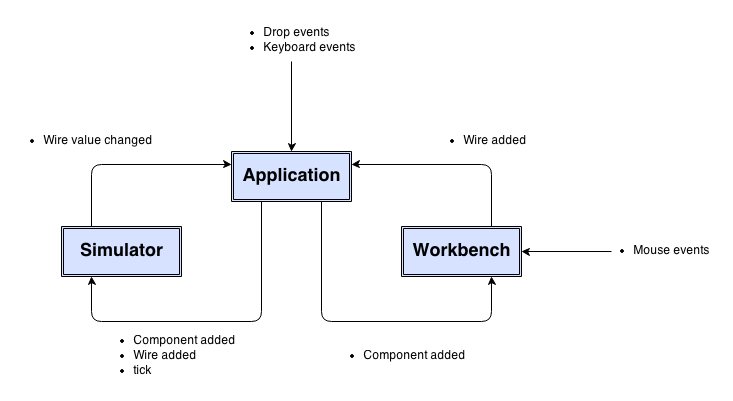
\includegraphics[width=\textwidth]{application.png}
    \caption{Information flow in GatePlay}
    \label{fig:application}
\end{figure}


\subsection{application.js}
